\documentclass[tikz]{standalone}


\usepackage{forest,xcolor}
\usetikzlibrary{matrix, positioning}

\begin{document}
  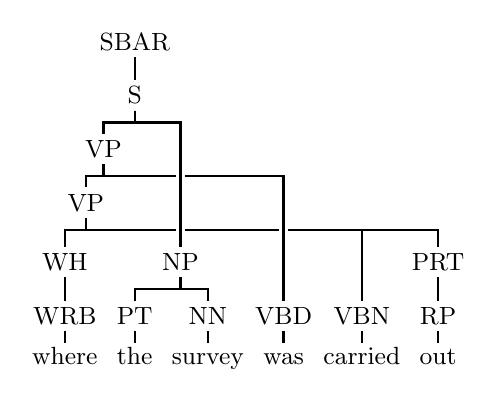
\begin{tikzpicture}[
      edge from parent path={(\tikzparentnode.south) -- ++(0,-1ex) -| (\tikzchildnode.north)},
      every path/.style={line width=.2ex},
      level distance=4.5ex,
%      node distance=3ex,
      anchor=center,
      every node/.style={font=\small}
    ]
    \matrix (pos) [matrix of nodes, outer sep=0pt, inner sep=0pt, row sep=0pt, column sep=7pt] {
      where\strut  & the\strut  & survey\strut   & was\strut  & carried\strut  & out\strut  \\};

    \node[fit=(pos-1-2) (pos-1-3), outer sep=0pt, inner sep=0pt] (npanc) {\strut};
    \begin{scope}[every node/.style={inner sep=2pt, font=\small}]
        \node[above=24ex of pos-1-2] (sbar) {SBAR}
        child { node (s) {S}
            child { node[xshift=1em] (vp1) {VP}
                child { node[xshift=1.5em] (vp2) {VP}
                    child { node[above=5.5ex of pos-1-1] (wh) {WH} child {
                            node[above=1ex of pos-1-1] (term0) {WRB}}}
                    child {
                        node[above=1ex of pos-1-5] (term4) {VBN}}
                    child { node[above=5.5ex of pos-1-6] (prt) {PRT} child {
                            node[above=1ex of pos-1-6] (term5) {RP}}}}
                child {
                    node[above=1ex of pos-1-4] (term3) {VBD}}
                edge from parent}
            child { node[above=5.5ex of npanc] (np) {NP}
                child { node[above=1ex of pos-1-2] (term1) {PT} }
                child {
                    node[above=1ex of pos-1-3] (term2) {NN}}}};
    \end{scope}
    \draw
        (term0) -- (pos-1-1)
        (term1) -- (pos-1-2)
        (term2) -- (pos-1-3)
        (term3) -- (pos-1-4)
        (term4) -- (pos-1-5)
        (term5) -- (pos-1-6);

     % redraw corssing edges with white foundation
     \begin{scope}
         \draw[white, line width=.7ex] (vp1.south) -- ++(0,-1ex) -| (term3.north);
         \draw (vp1.south) -- ++(0,-1ex) -| (vp2.north);
         \draw (vp1.south) -- ++(0,-1ex) -| (term3.north);

         \draw[white, line width=.7ex] (s.south) ++(.5pt,-.5ex) -| (np.north);
         \draw (s.south) -- ++(0,-1ex) -| (np.north);
         \draw (s.south) -- ++(0,-1ex) -| (vp1.north);
     \end{scope}
  \end{tikzpicture}
\end{document}
